\section{Dataset utilizzato}
Il dataset utilizzato per il progetto è stato prelevato dal sito \cite{dataset_site}, che mette a disposizione i dati di train ($12060$ \textit{sample}) e di test ($647$ \textit{sample}) per lo svolgimento della \textit{challenge}.
Ogni elemento del dataset rappresenta un differente composto chimico ed è caratterizzato da un insieme di $801$ feature dense e oltre $200000$ feature sparse. Considerata la complessità computazionale aggiuntiva derivante dall'utilizzo di queste ultime feature a fronte della minima quantità di informazione apportata, è stato deciso di non considerare la porzione sparsa della matrice, come consigliato dai \textit{publisher} del dataset.
Ad ogni \textit{sample} è associato un vettore binario di etichette contenente $12$ elementi; ognuno di essi corrisponde al risultato di una differente analisi tossicologica a cui la molecola è stata sottoposta.

L'analisi della matrice delle etichette ha mostrato una discreta presenza di valori \texttt{NaN} (35\% nel train set, 10\% nel test set); non essendo presente alcuna motivazione circa la presenza di questi valori nella descrizione del dataset, è stato supposto che alcune analisi siano state tralasciate per quelle molecole che i ricercatore hanno ritenuto certamente non tossiche in determinati \textit{pathways}. Per questo motivo, i valori \texttt{NaN} sono stati sostituiti con $0$, rappresentando quindi un esito del test tossicologico negativo per il composto chimico associato.
\begin{figure}[!ht]
	\centering
	\subfloat{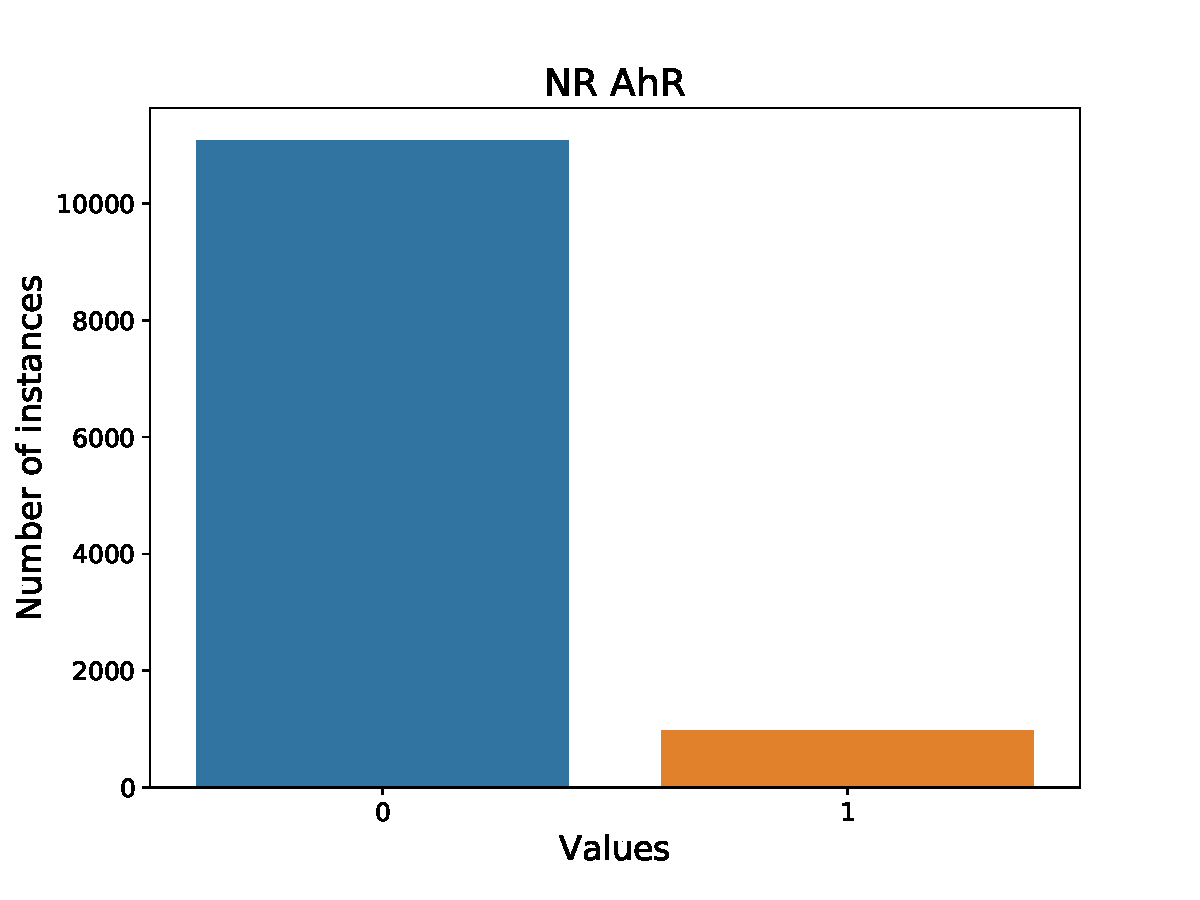
\includegraphics[width=.2\textwidth]{../images/pdf/hist-NRAhR}}\quad
	\subfloat{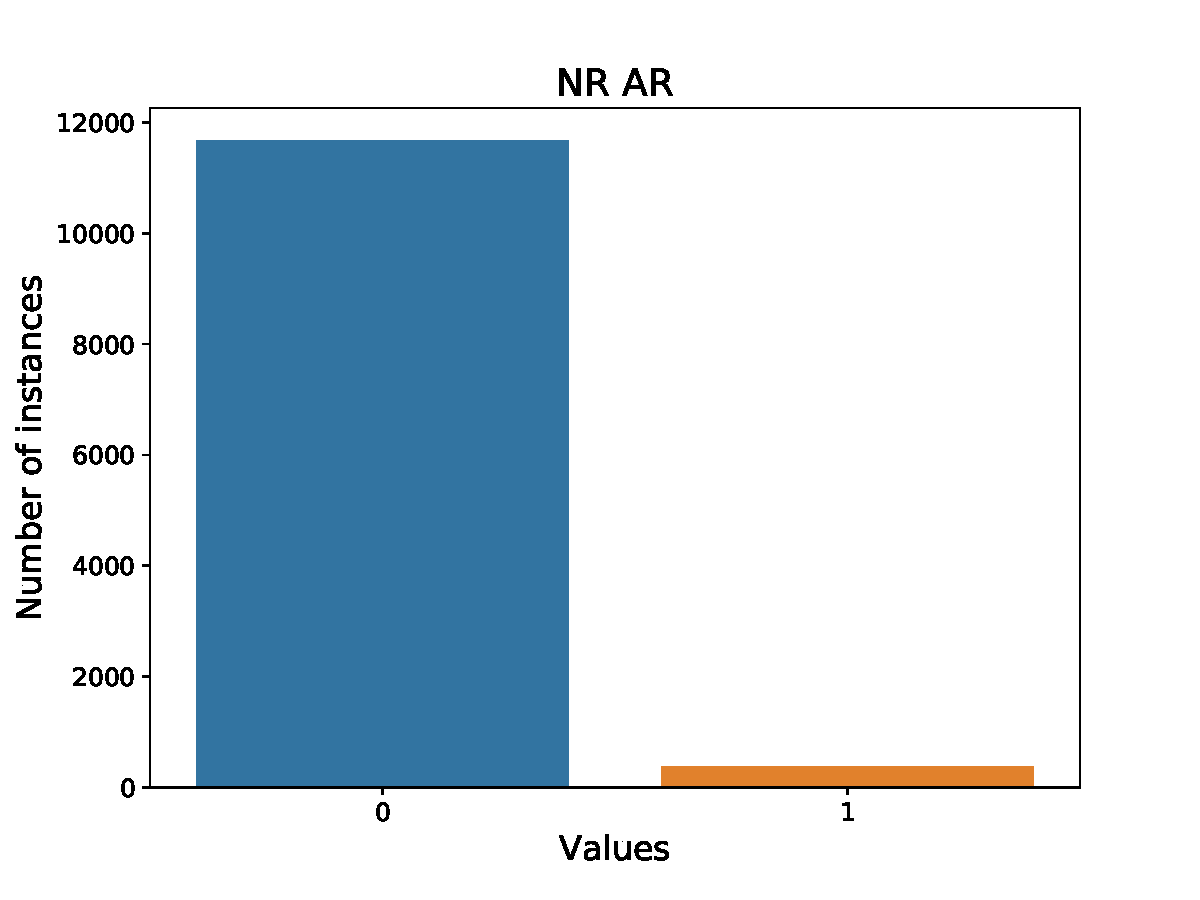
\includegraphics[width=.2\textwidth]{../images/pdf/hist-NRAR}}\quad
	\subfloat{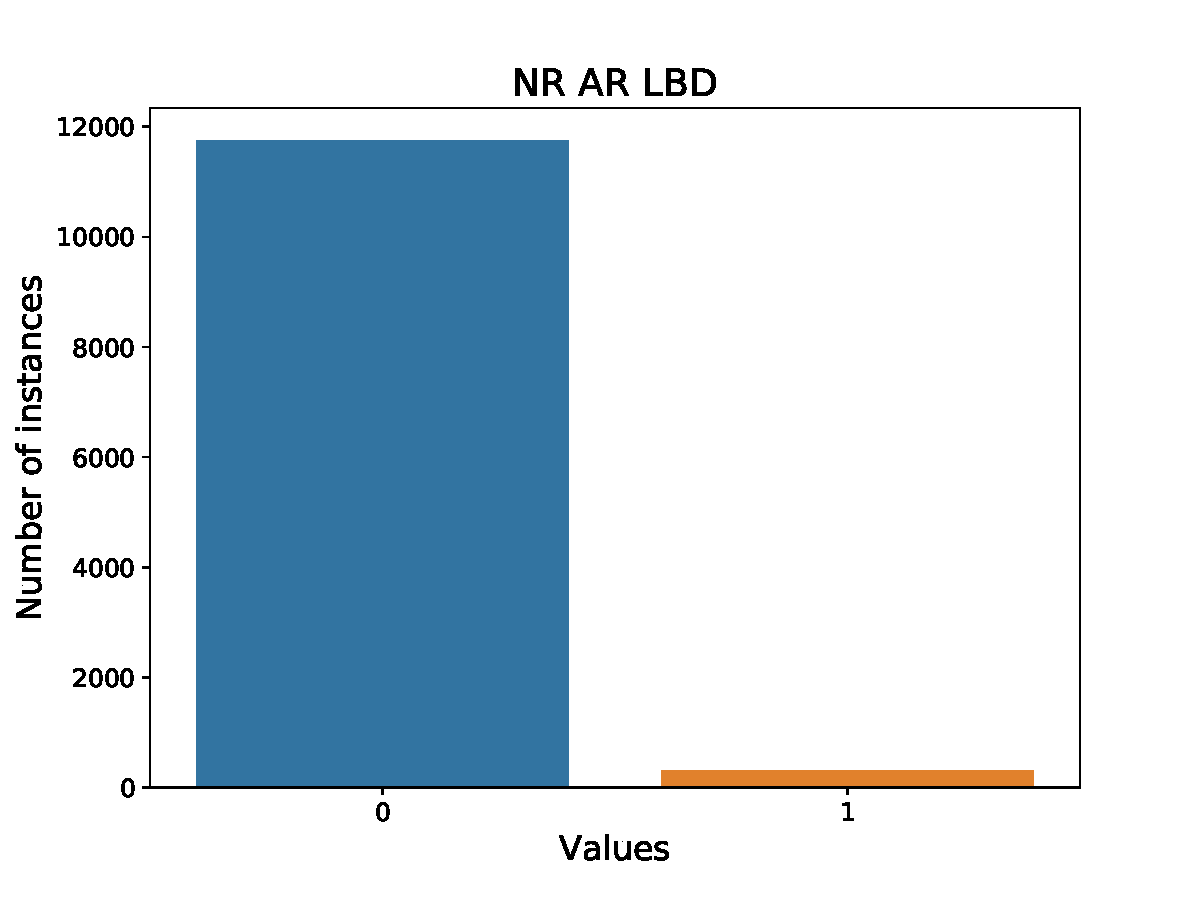
\includegraphics[width=.2\textwidth]{../images/pdf/hist-NRARLBD}}\quad
	\subfloat{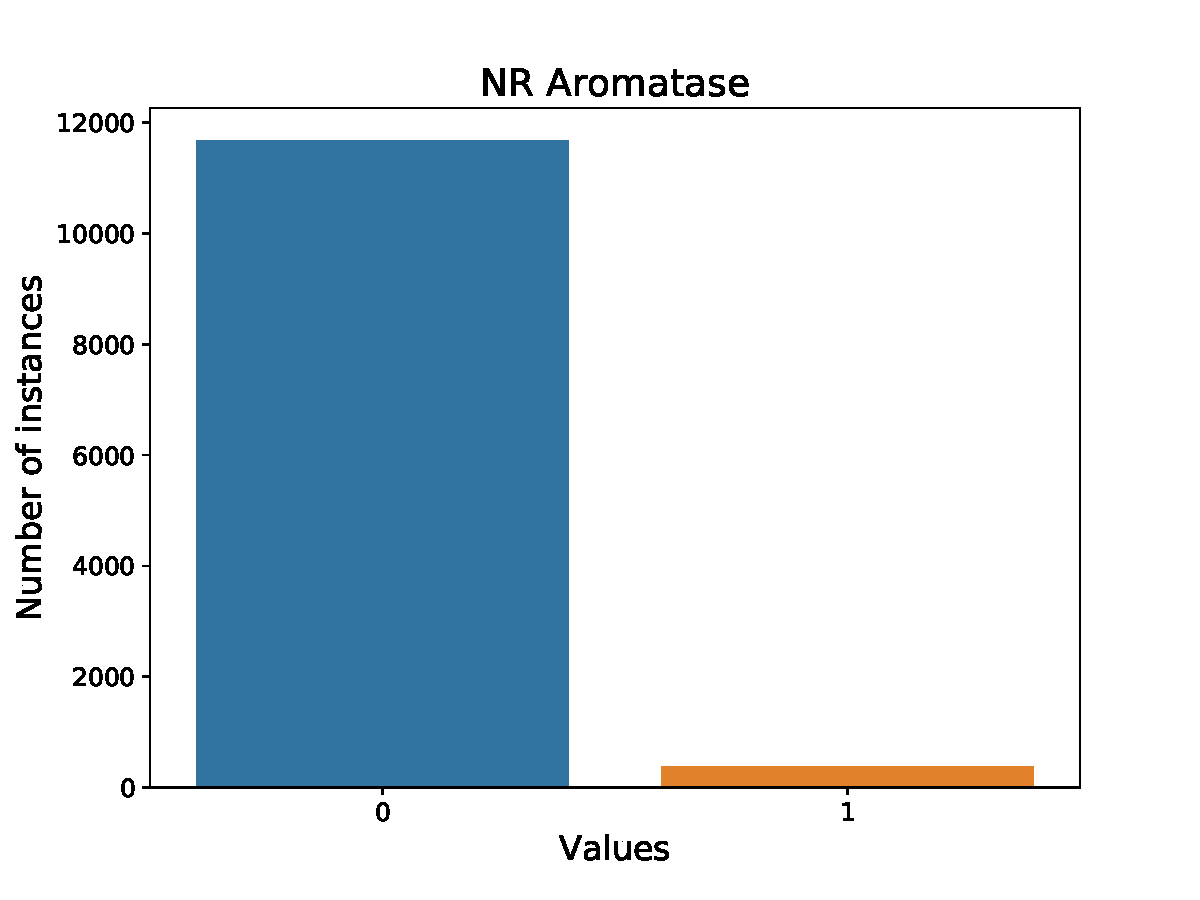
\includegraphics[width=.2\textwidth]{../images/pdf/hist-NRAromatase}}\\	\subfloat{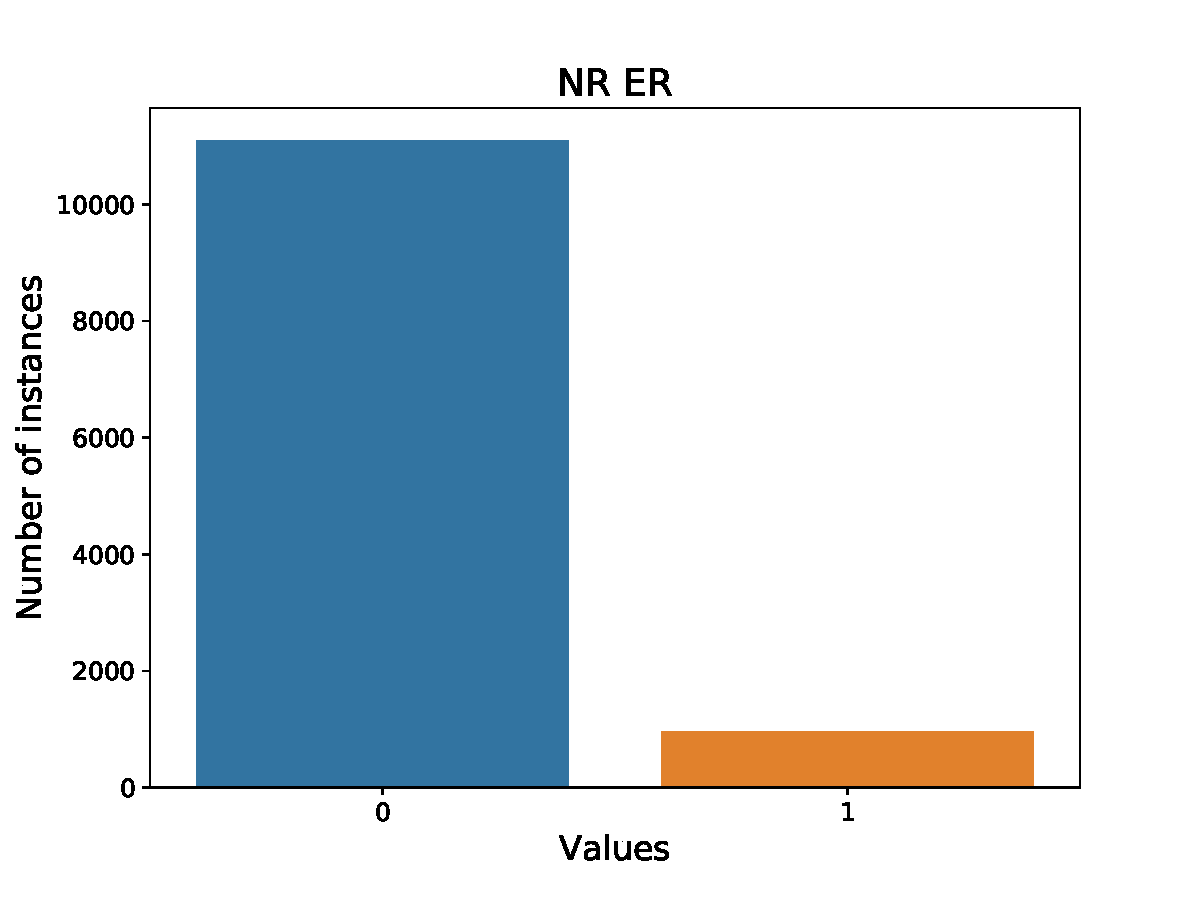
\includegraphics[width=.2\textwidth]{../images/pdf/hist-NRER}}\quad
	\subfloat{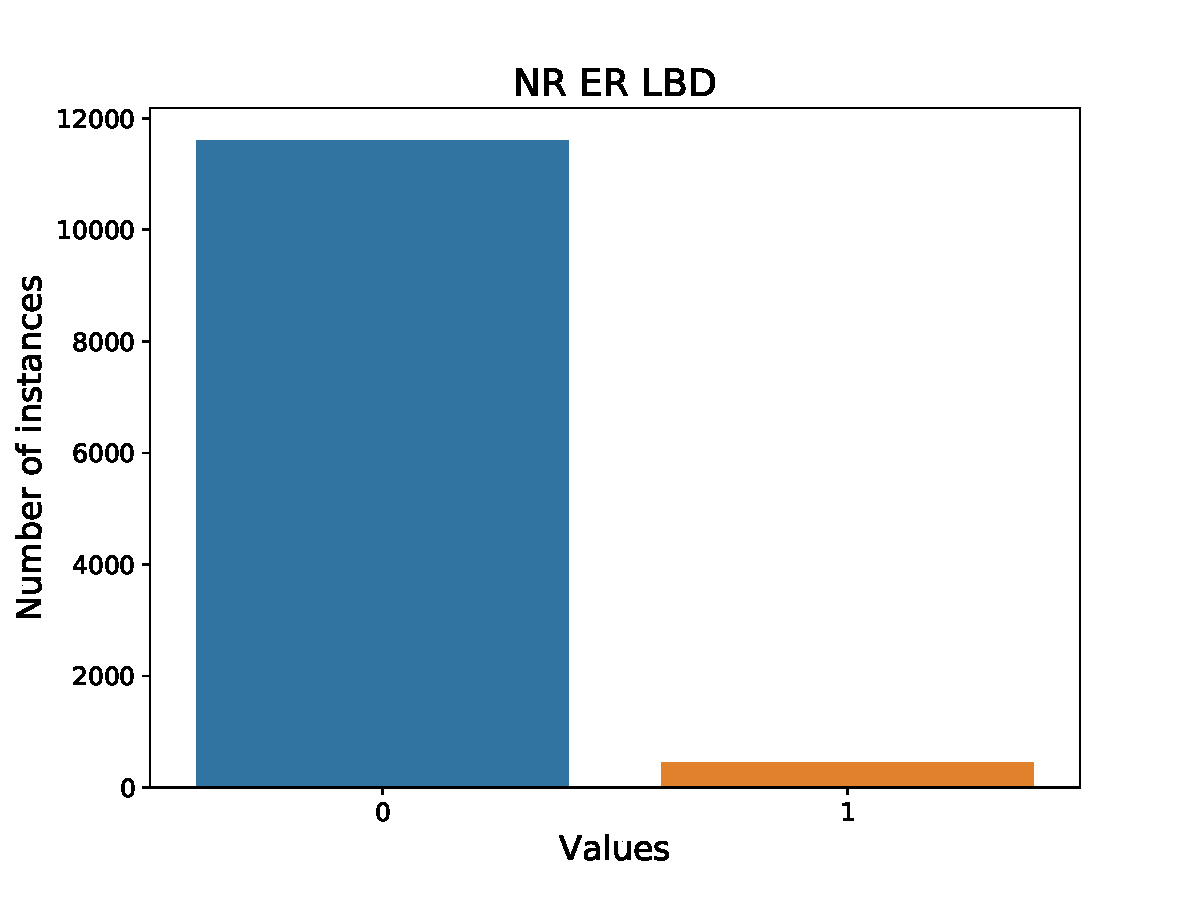
\includegraphics[width=.2\textwidth]{../images/pdf/hist-NRERLBD}}\quad
	\subfloat{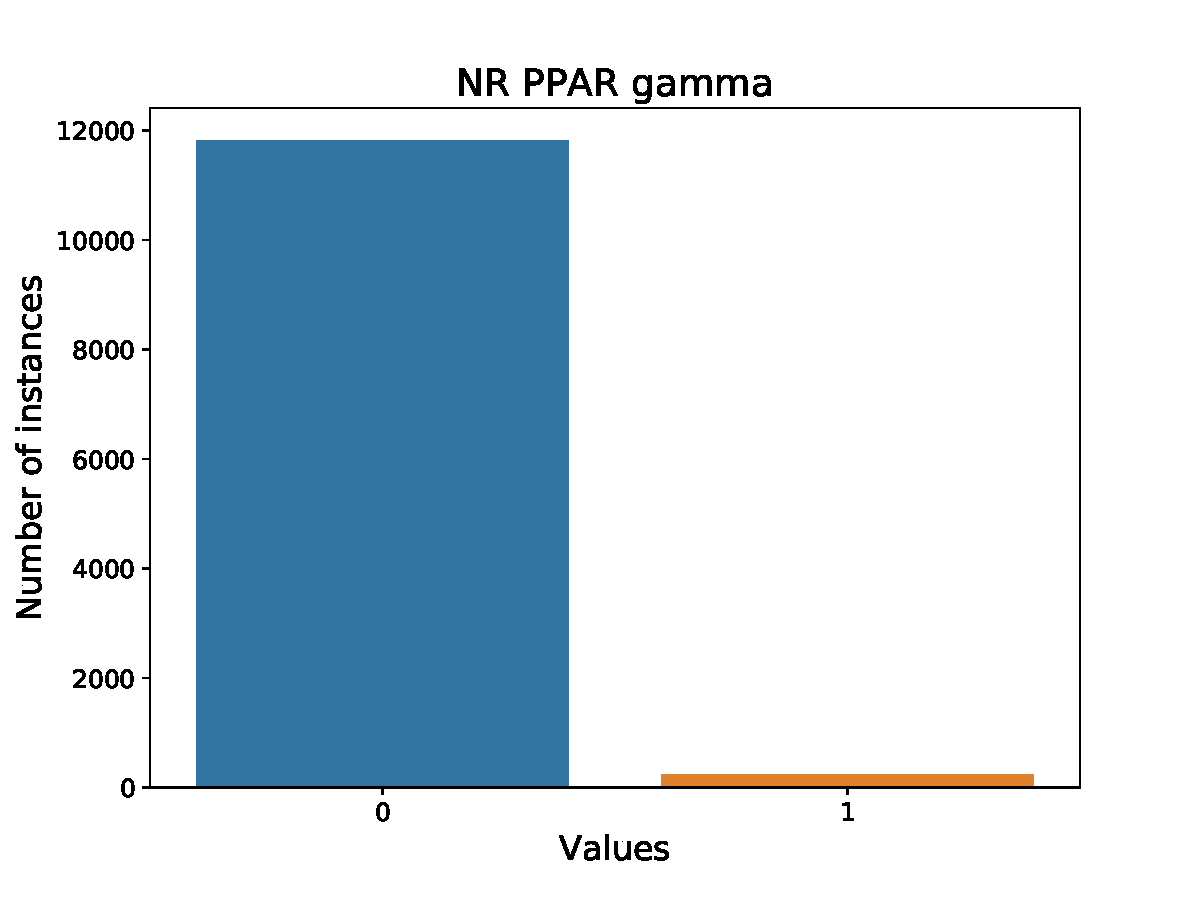
\includegraphics[width=.2\textwidth]{../images/pdf/hist-NRPPARgamma}}\quad
	\subfloat{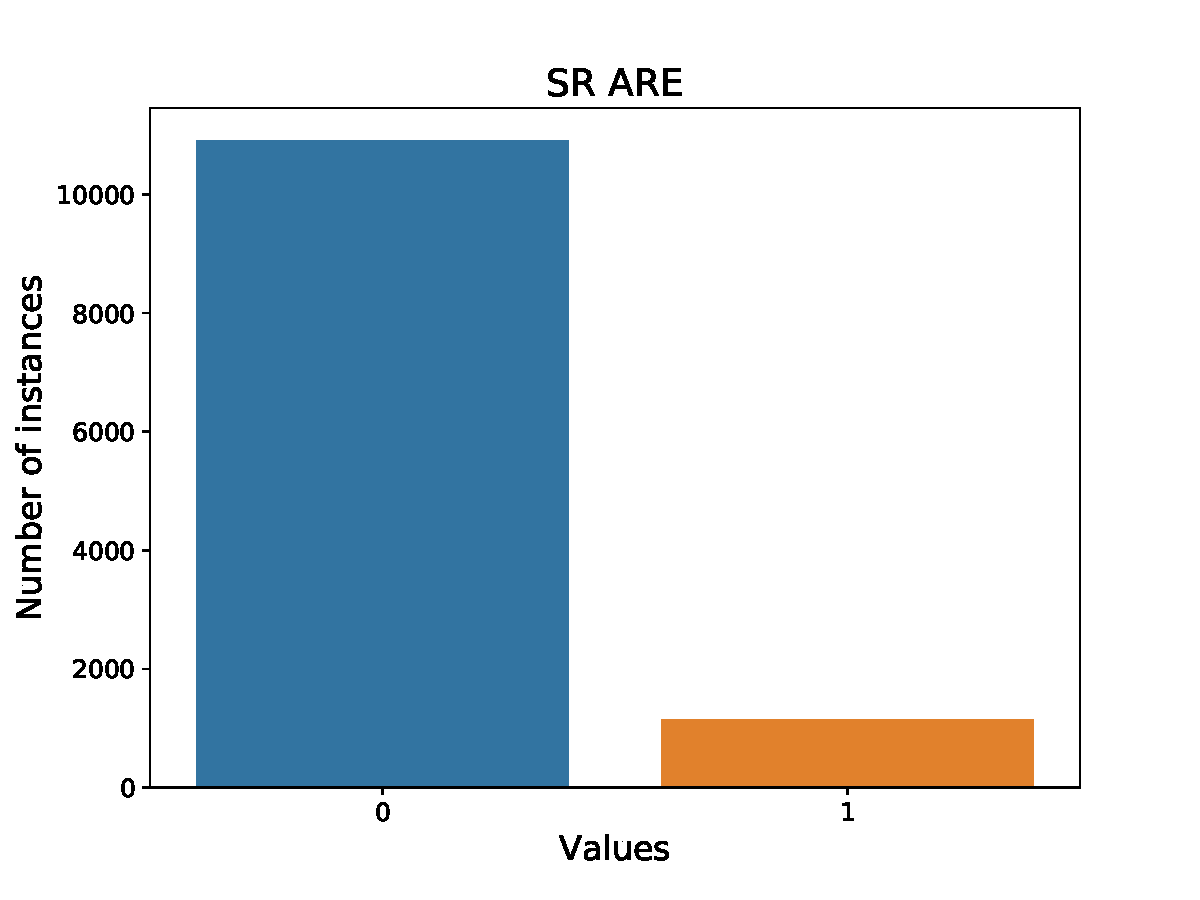
\includegraphics[width=.2\textwidth]{../images/pdf/hist-SRARE}}\\
	\subfloat{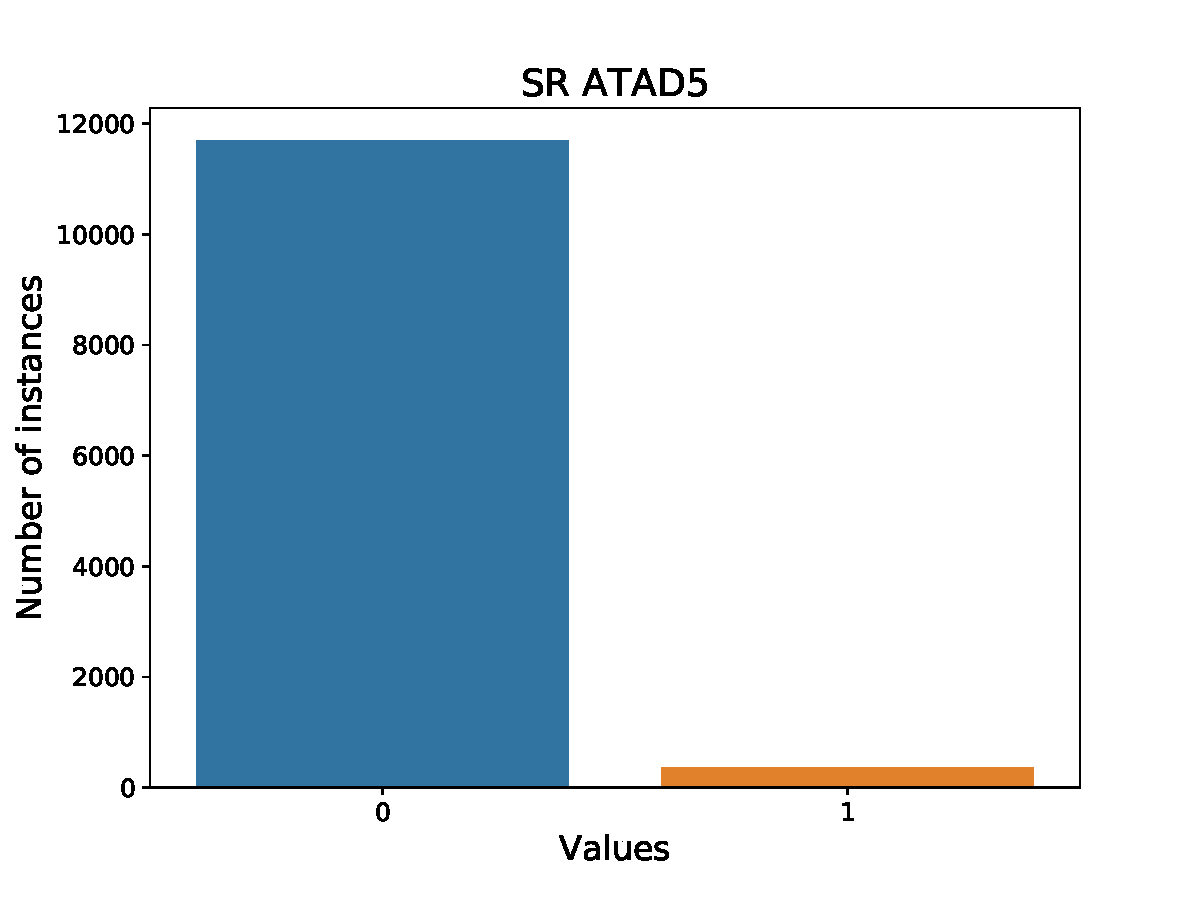
\includegraphics[width=.2\textwidth]{../images/pdf/hist-SRATAD5}}\quad
	\subfloat{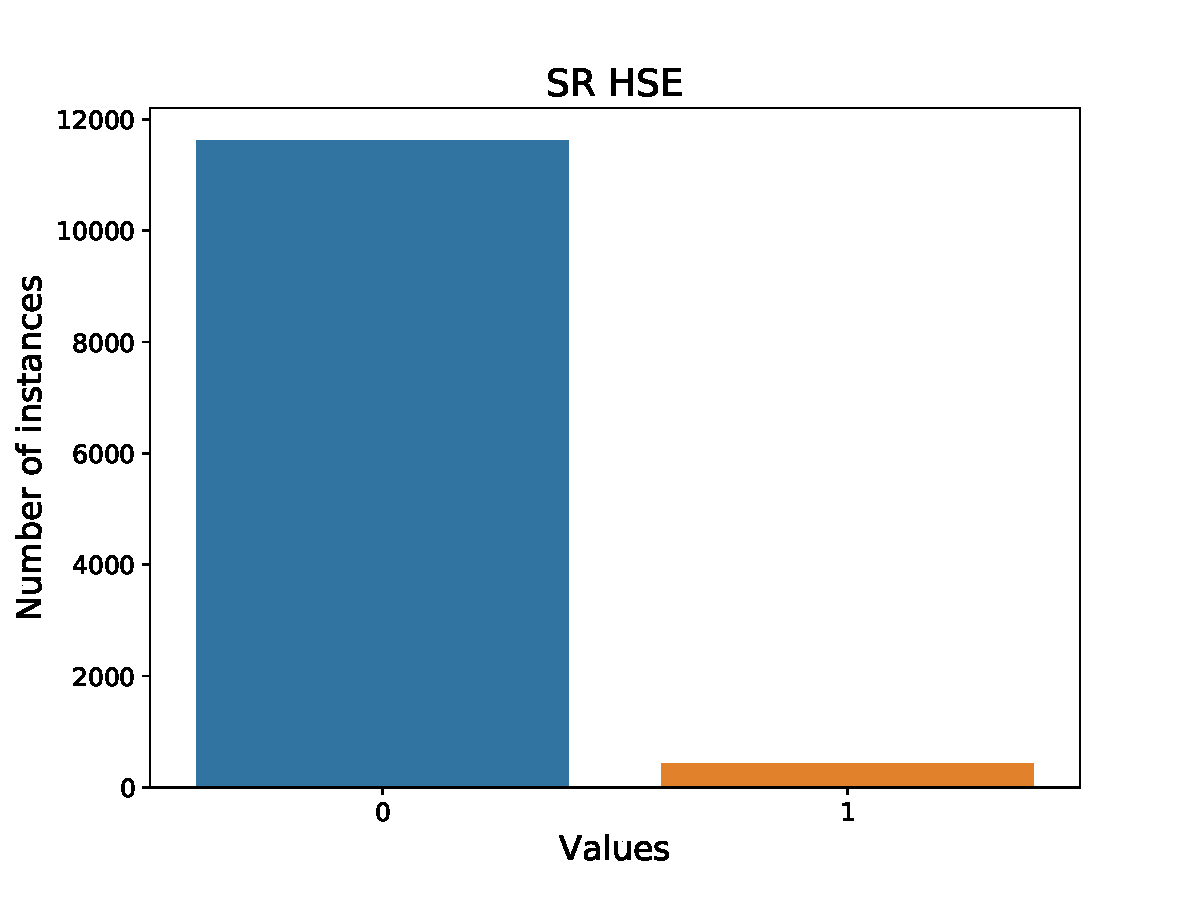
\includegraphics[width=.2\textwidth]{../images/pdf/hist-SRHSE}}\quad	\subfloat{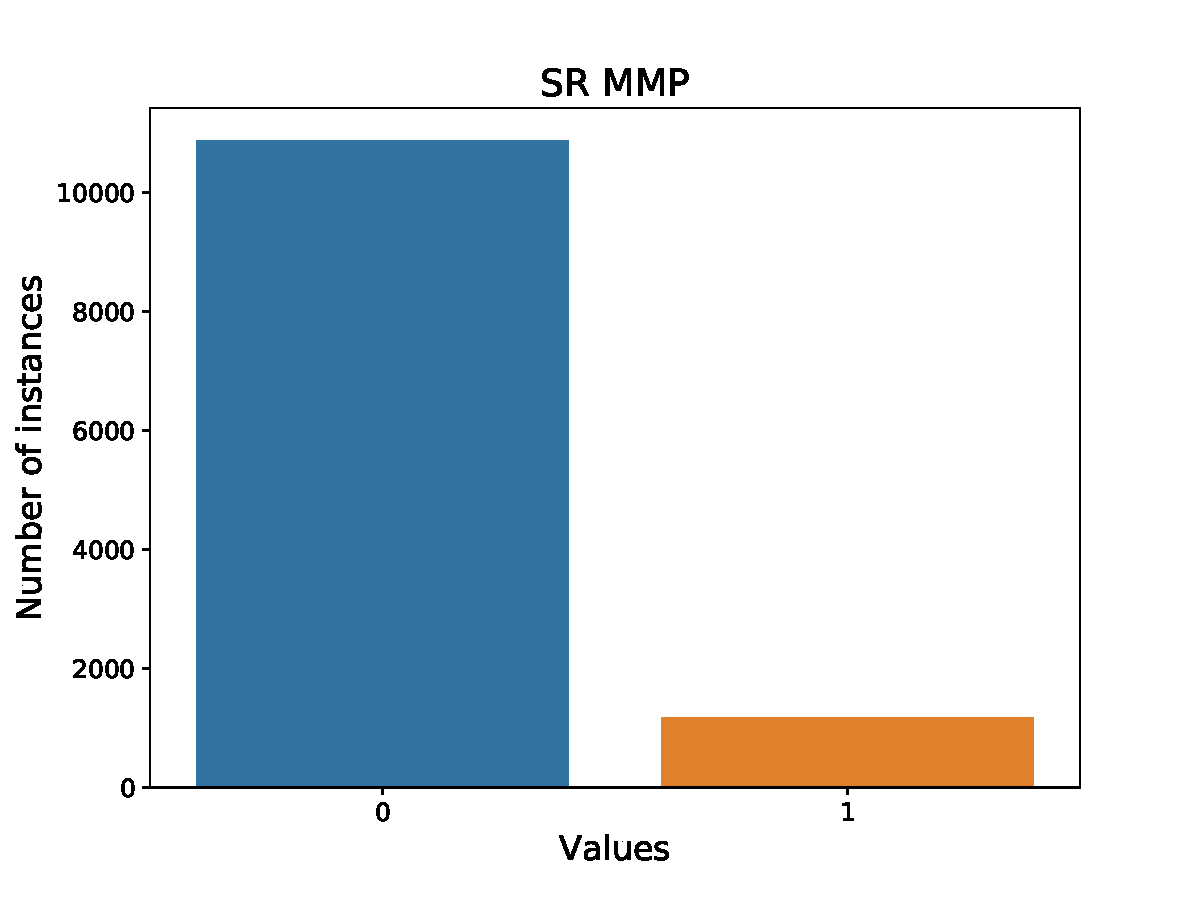
\includegraphics[width=.2\textwidth]{../images/pdf/hist-SRMMP}}\quad
	\subfloat{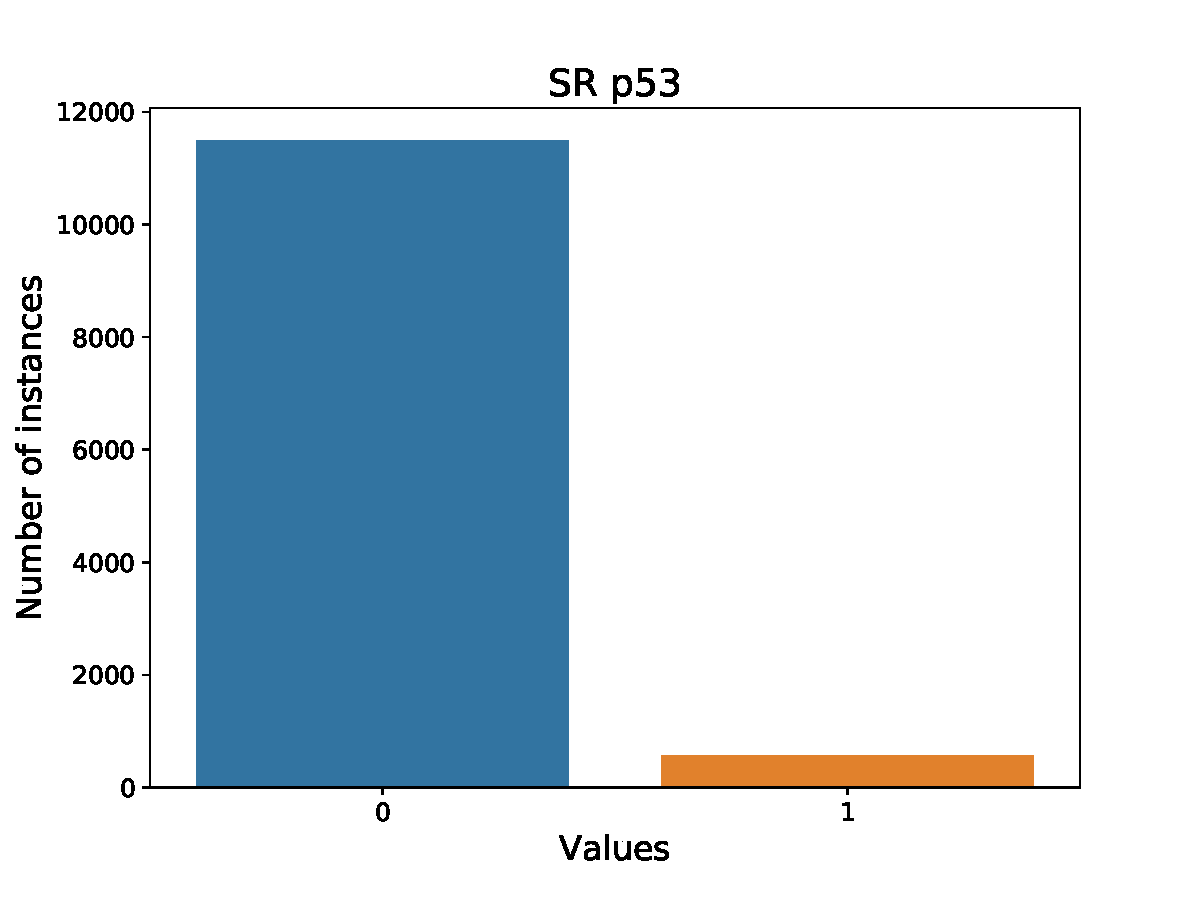
\includegraphics[width=.2\textwidth]{../images/pdf/hist-SRp53}}
	\caption{Distribuzione delle etichette dei differenti test tossicologici.}
	\label{fig:class_distribution}
\end{figure}
\\L'attenzione è stata poi spostata sull'analisi della distribuzione delle etichette, riportata in Figura \ref{fig:class_distribution}, che mostra un forte sbilanciamento tra il numero di 0 ed il numero di 1 per ogni classe. 
Data la natura multi-label del problema, per avendo rilevato lo sbilanciamento presente tra le classi, non è stato possibile effettuare operazioni di \textit{over/under-sampling}, in quanto la generazione di un nuovo \textit{sample} sintetico (o la rimozione di un record nel caso complementare) per una classe avrebbe influenzato lo sbilanciamento delle classi rimanenti.
L'analisi della correlazione tra le etichette è stata indagata mediante una rappresentazione \textit{heatmap} della matrice di correlazione, riportata in Figura \ref{fig:labelscorrmatrixheatmap}.
I valori di correlazione risultano essere molto bassi in media, salvo qualche eccezione. 
Analizzando la semantica delle etichette, è emerso che le due coppie di label correlate in modo significativo riguardano la tossicità in un caso sull'intero recettore, nell'altro solo su una porzione di esso.
\begin{figure}
	\begin{tabular}{cc}
		\subfloat[\label{fig:labelscorrmatrixheatmap}\textit{Heatmap} della matrice di correlazione delle label.]{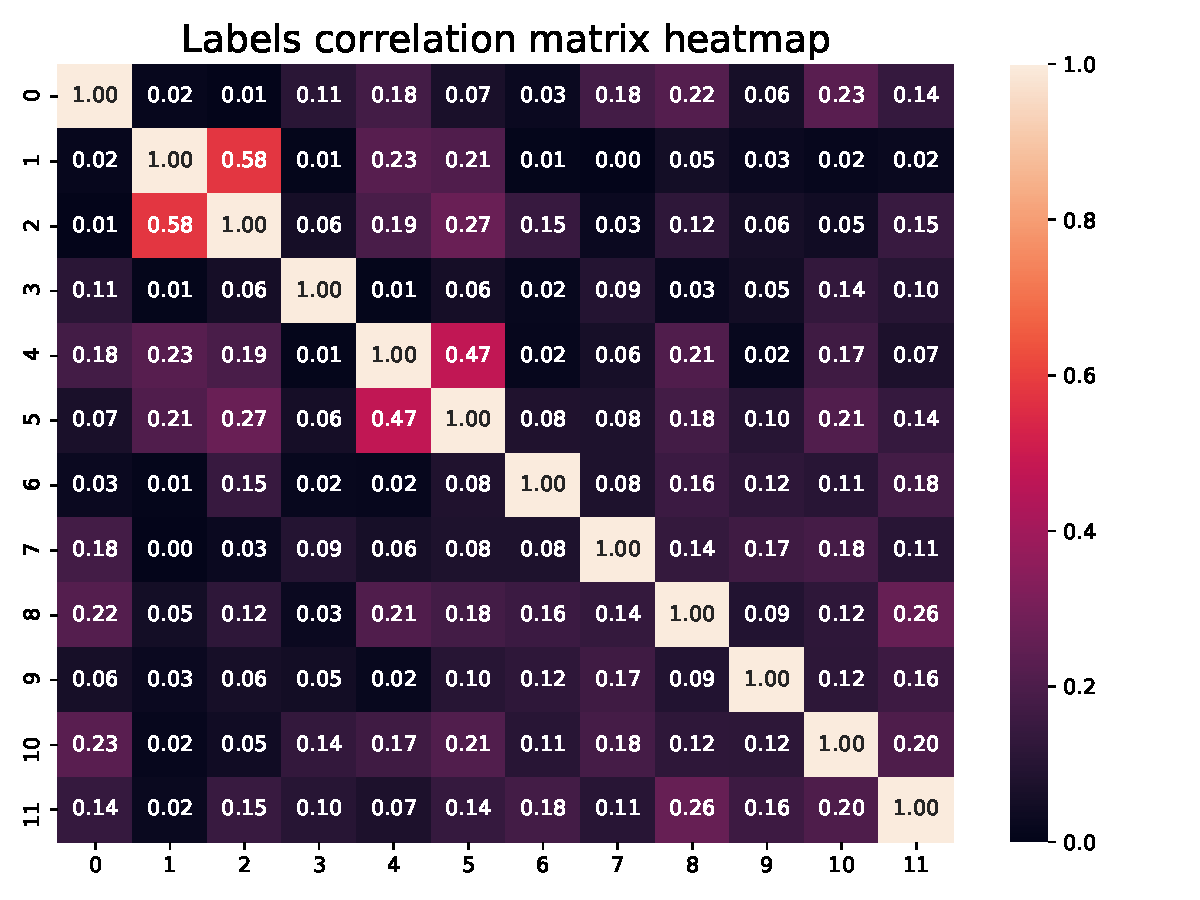
\includegraphics[width = .5\textwidth]{../images/pdf/labels_corr_matrix_heatmap}} &
		\subfloat[\label{fig:distributionhighcorr}Distribuzione di feature/label altamente correlate. È stata utilizzata la scala logaritmica per l'asse \textit{x}.]{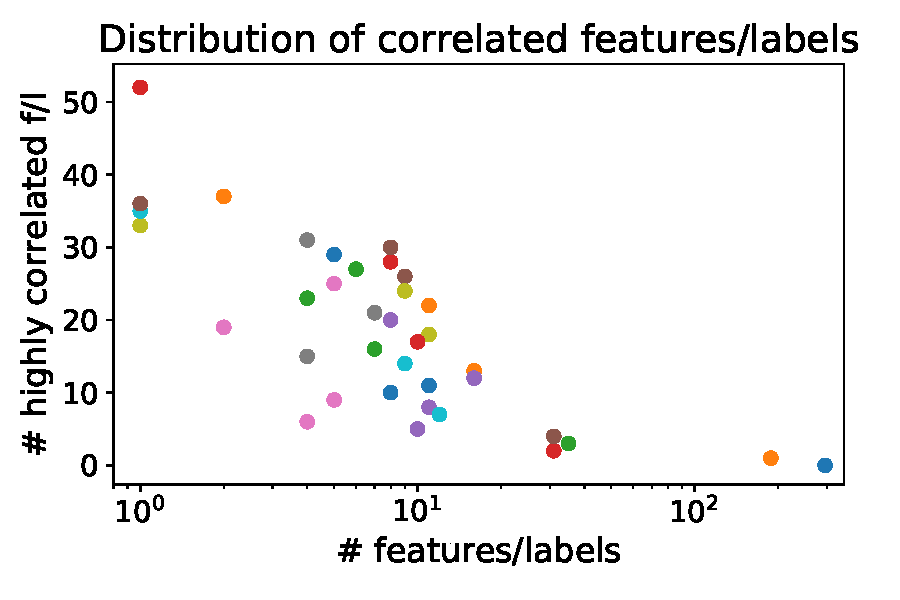
\includegraphics[width = .5\textwidth]{../images/pdf/distribution_high_corr}} 
	\end{tabular}
	\caption{In Figura sono riportate come le label sono correlate tra loro (Figura \ref{fig:labelscorrmatrixheatmap}) e come si distribuiscono le feature/label in base a con quante altre feature/label sono altamente correlate tra loro (Figura \ref{fig:distributionhighcorr}).}
\end{figure} 
Per quanto riguarda le feature, è stata verificata la presenza di \textit{missing value} e il tipo dei dati contenuti nella matrice delle feature. 
L'analisi non ha evidenziato la presenza di alcun valore mancante e i dati si sono rivelati tutti di tipo numerico.
Successivamente, sono state eseguite alcune operazioni di pulizia del dataset, rimuovendo $7$ feature con varianza pari a $0$ e $425$ \textit{sample} considerati come outlier; sono stati identificati come outlier quei \textit{sample} che avessero almeno $\frac{1}{4}$ dei valori che eccedessero $3$ volte lo scarto interquantile delle relative feature.
L'analisi della correlazione tra feature e label non ha mostrato la presenza di feature altamente correlate alle label, con un valore di correlazione massimo pari a $0.35$; le feature maggiormente correlate alle diverse etichette si sono inoltre rivelate essere tutte differenti (tranne in un caso), rafforzando l'ipotesi dell'assenza di uno stretto legame tra le etichette e un'unica feature.
In Figura \ref{fig:distributionhighcorr}, è riportata un'analisi di come le varie feature/etichette sono risultate altamente correlate ($> 0.90$) con altre feature/etichette. 
È possibile vedere come la larga maggioranza degli elementi sia correlato con un basso numero di feature.
Si rilevano poi un insieme di feature correlate con un numero di elementi compreso tra $5$ e $30$, mentre una decina di feature risultano correlate a più di 40 elementi. 
Questo suggerisce che sia opportuno eseguire un'operazione di feature reduction prima di eseguire l'addestramento del modello, in modo da ridurre la ridondanza di informazione e aumentando così il potenziale di generalizzazione del modello.
Infine, i dati sono stati standardizzati con media nulla e deviazione standard unitaria, in modo da non creare squilibri, in termini di magnitudine dell'input dei modelli neurali presentati nelle prossime sezioni.%; ciò è stato fatto in quanto feature con scale differenti possono portare instabilità nella rete, causando la creazione di pesi troppo elevati che rendono le predizioni fortemente suscettibili a piccole variazioni dell'input.